\documentclass[12pt,tikz]{standalone}
 
\usepackage{tkz-euclide}
\usetikzlibrary{shapes,backgrounds}

\usetikzlibrary{snakes}

\newcommand\Star[3][]{%
		\path[#1] (0  :#3) -- ( 36:#2) 
		-- (72 :#3) -- (108:#2)
		-- (144:#3) -- (180:#2)
		-- (216:#3) -- (252:#2)
		-- (288:#3) -- (324:#2)--cycle;
	}
\newcommand\Center[3][]{
	\begin{scope}[shift = {(#2,#3)}, scale=0.08]
		\Star[#1]{2}{4}
	\end{scope}
	}
	
\newcommand\point[3][]{
	\begin{scope}[shift = {(#2,#3)}, scale=0.08]
		\draw[#1] (0,0) circle (1.5);
	\end{scope}
	}
 
\begin{document}
		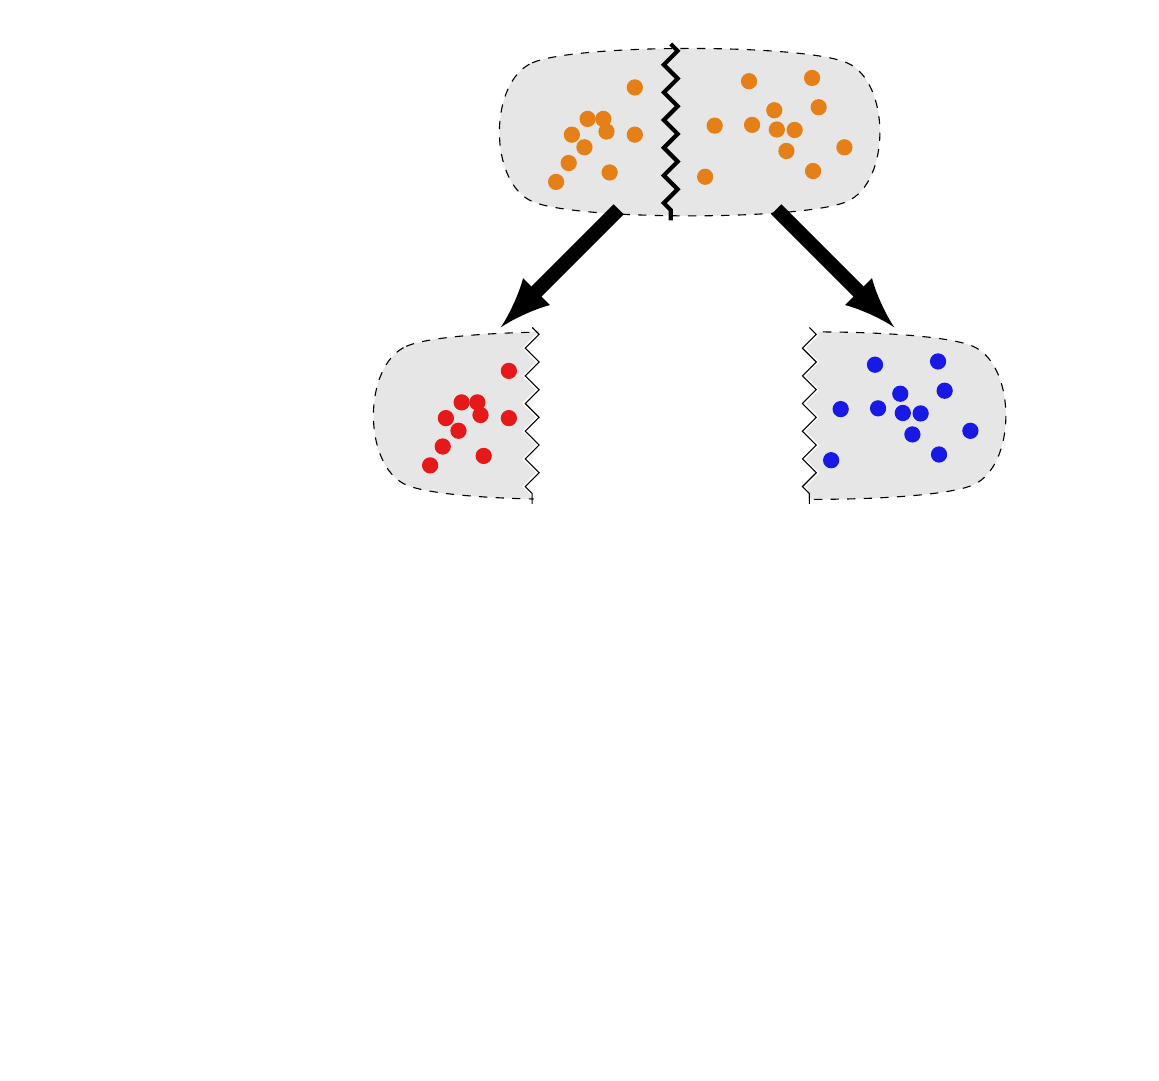
\begin{tikzpicture}[scale=1]

			\tkzInit[xmax=22,ymax=11,xmin=8,ymin=-2]
			\begin{scope}[dash pattern=on 0pt off 4pt]
			\tkzGrid
			\end{scope}

			\begin{scope}[scale=0.8, yshift=3cm, xshift=2cm]
			
			\begin{scope}[yshift=7cm, xshift=5cm]
			\point[fill=orange, draw=orange]{2.13}{2.31}
			\point[fill=orange, draw=orange]{2.63}{2.81}
			\point[fill=orange, draw=orange]{1.88}{2.31}
			\point[fill=orange, draw=orange]{2.63}{2.06}
			\point[fill=orange, draw=orange]{2.23}{1.46}
			\point[fill=orange, draw=orange]{1.58}{1.6099999999999999}
			\point[fill=orange, draw=orange]{1.63}{2.06}
			\point[fill=orange, draw=orange]{1.38}{1.31}
			\point[fill=orange, draw=orange]{2.1799999999999997}{2.1100000000000003}
			\point[fill=orange, draw=orange]{1.83}{1.8599999999999999}
			
			\begin{scope}[yshift=-4.5cm,xshift=-2cm]
					\point[fill=red, draw=red]{2.13}{2.31}
					\point[fill=red, draw=red]{2.63}{2.81}
					\point[fill=red, draw=red]{1.88}{2.31}
					\point[fill=red, draw=red]{2.63}{2.06}
					\point[fill=red, draw=red]{2.23}{1.46}
					\point[fill=red, draw=red]{1.58}{1.6099999999999999}
					\point[fill=red, draw=red]{1.63}{2.06}
					\point[fill=red, draw=red]{1.38}{1.31}
					\point[fill=red, draw=red]{2.1799999999999997}{2.1100000000000003}
					\point[fill=red, draw=red]{1.83}{1.8599999999999999}
			\end{scope}

			\begin{scope}[yshift=-1.5cm, xshift=-3.7cm]
				\point[fill=orange, draw=orange]{9.14345684}{4.460019389999999}
				\point[fill=orange, draw=orange]{8.86688485}{3.63473389}
				\point[fill=orange, draw=orange]{7.59755558}{3.70343663}
				\point[fill=orange, draw=orange]{8.191160570000001}{3.71538839}
				\point[fill=orange, draw=orange]{9.15882059}{2.98267676}
				\point[fill=orange, draw=orange]{7.44631872}{2.8917449299999998}
				\point[fill=orange, draw=orange]{9.24811186}{3.99537327}
				\point[fill=orange, draw=orange]{9.65681417}{3.35879586}
				\point[fill=orange, draw=orange]{8.583686310000001}{3.64166512}
				\point[fill=orange, draw=orange]{8.54357414}{3.94752138}
				\point[fill=orange, draw=orange]{8.142720709999999}{4.408464840000001}
				\point[fill=orange, draw=orange]{8.736270430000001}{3.30132992}
			\end{scope}
			
			\begin{scope}[yshift=-4.5cm,xshift=2cm]
				\begin{scope}[yshift=-1.5cm, xshift=-3.7cm]
				\point[fill=blue, draw=blue]{9.14345684}{4.460019389999999}
				\point[fill=blue, draw=blue]{8.86688485}{3.63473389}
				\point[fill=blue, draw=blue]{7.59755558}{3.70343663}
				\point[fill=blue, draw=blue]{8.191160570000001}{3.71538839}
				\point[fill=blue, draw=blue]{9.15882059}{2.98267676}
				\point[fill=blue, draw=blue]{7.44631872}{2.8917449299999998}
				\point[fill=blue, draw=blue]{9.24811186}{3.99537327}
				\point[fill=blue, draw=blue]{9.65681417}{3.35879586}
				\point[fill=blue, draw=blue]{8.583686310000001}{3.64166512}
				\point[fill=blue, draw=blue]{8.54357414}{3.94752138}
				\point[fill=blue, draw=blue]{8.142720709999999}{4.408464840000001}
				\point[fill=blue, draw=blue]{8.736270430000001}{3.30132992}
				\end{scope}
			\end{scope}
			

			\draw [black, fill=white!50!black, fill opacity=0.2, dash pattern=on 3pt off 3pt] plot [smooth cycle, tension=.5] coordinates {(1,1) (1,3.2) (6,3.2) (6,1)};		
			\begin{scope}[line width=1.5pt]
			\draw[snake=zigzag, draw=black] (3.2,3.5) -- (3.2,0.7);
			\end{scope}	
%			\draw[snake=zigzag, draw=black] (3.0,3.5) -- (3.0,0.7);
%			\draw[snake=zigzag, draw=black] (3.4,3.5) -- (3.4,0.7);	
			\end{scope}
			\end{scope}
			
			\begin{scope}[scale=0.8, xshift=5cm, yshift=5.5cm]
				\draw [black, fill=white!50!black, fill opacity=0.2, dash pattern=on 3pt off 3pt] plot [smooth cycle, tension=.5] coordinates {(1,1) (1,3.2) (6,3.2) (6,1)};		
				\begin{scope}[line width=8pt]
				\draw[snake=zigzag, draw=white] (3.2,3.5) -- (3.2,0.7);
				\end{scope}	
				\draw[snake=zigzag, draw=black] (3.0,3.5) -- (3.0,0.7);
				\draw[snake=zigzag, draw=black] (3.4,3.5) -- (3.4,0.7);	
				\draw [fill=white, draw=none] (3.2,0.5) rectangle ++(3.7,3.2);
			\end{scope}
			
						
			\begin{scope}[scale=0.8, xshift=9cm, yshift=5.5cm]
				\draw [black, fill=white!50!black, fill opacity=0.2, dash pattern=on 3pt off 3pt] plot [smooth cycle, tension=.5] coordinates {(1,1) (1,3.2) (6,3.2) (6,1)};		
				\begin{scope}[line width=8pt]
				\draw[snake=zigzag, draw=white] (3.2,3.5) -- (3.2,0.7);
				\end{scope}	
				\draw[snake=zigzag, draw=black] (3.0,3.5) -- (3.0,0.7);
				\draw[snake=zigzag, draw=black] (3.4,3.5) -- (3.4,0.7);	
				\draw [fill=white, draw=none] (3.2,0.5) rectangle ++(-3.7,3.2);
			\end{scope}
			
			
			\begin{scope}[yshift=7.2cm,xshift=6cm]
			\begin{scope}[xshift=0cm]
			\pgfsetarrowsstart{latex}
			\pgfsetlinewidth{1.2ex}
			\pgfpathmoveto{\pgfpointorigin}
			\pgfpathlineto{\pgfpoint{1.5cm}{1.5cm}}
			\pgfusepath{stroke}
			\end{scope}
			
			\begin{scope}[xshift=5cm]
			\pgfsetarrowsstart{latex}
			\pgfsetlinewidth{1.2ex}
			\pgfpathmoveto{\pgfpointorigin}
			\pgfpathlineto{\pgfpoint{-1.5cm}{1.5cm}}
			\pgfusepath{stroke}
			\end{scope}
			\end{scope}
%			\end{scope}
			
			
			
			%%%%%%%%%%%%%%%%%%%%%%%%%%%%%%%%%%%%%%%%%%%%%%%%%%%%%%%
			
			
		\end{tikzpicture}
\end{document}